The validation of the maximum likelihood fit, used to extract all information in this
analysis, is now described. The validation procedure consists of
two main tests. The first test is a fit using a data sample without
anomalous couplings. Such a test allows to identify problems with
event generation causing discrepancies in the leading lepton
\pt\ distribution. The second test is a fit using a data sample with
anomalous couplings. Such a test checks if we can properly measure
anomalous couplings when they are present. Both tests are critical to
validate the fitting tools, which are fairly complicated.

In the previous analysis it was found that the leading lepton
\pt\ distribution does not allow to differentiate between different
couplings and a typical observation inconsistent with Standard Model
represents a class of possible coupling values.

Figure~\ref{fig:val_scans} shows fit results and likelihood scans for
\ww\ simulated data with and without anomalous couplings. One may
conclude that even though the fit was able to measure the couplings
close to the true values, there is large uncertainty on the angle
between the two couplings as is revealed in the shapes of the contour
plots in the likelihood scans.

Figure~\ref{fig:lz_vs_dkg} shows what effect different anomalous
couplings have on the shape of the leading lepton \pt{}. It is
important to notice that relative effect of anomalous couplings
depends on the coupling, which affects sensitivity of the search. In
particular two of the most sensitive couplings, $\lambda_{Z}$ and
$\Delta g^Z_1$, differ significantly in the tail of the leading
lepton \pt{}. Comparing cross-sections from Table~\ref{tab:xsections}
one can conclude that $\Delta g^Z_1$ needs roughly 50\% stronger
coupling to produce an effect similar to that of $\lambda_{Z}$.

\begin{figure}[tp]
  \centerline{
    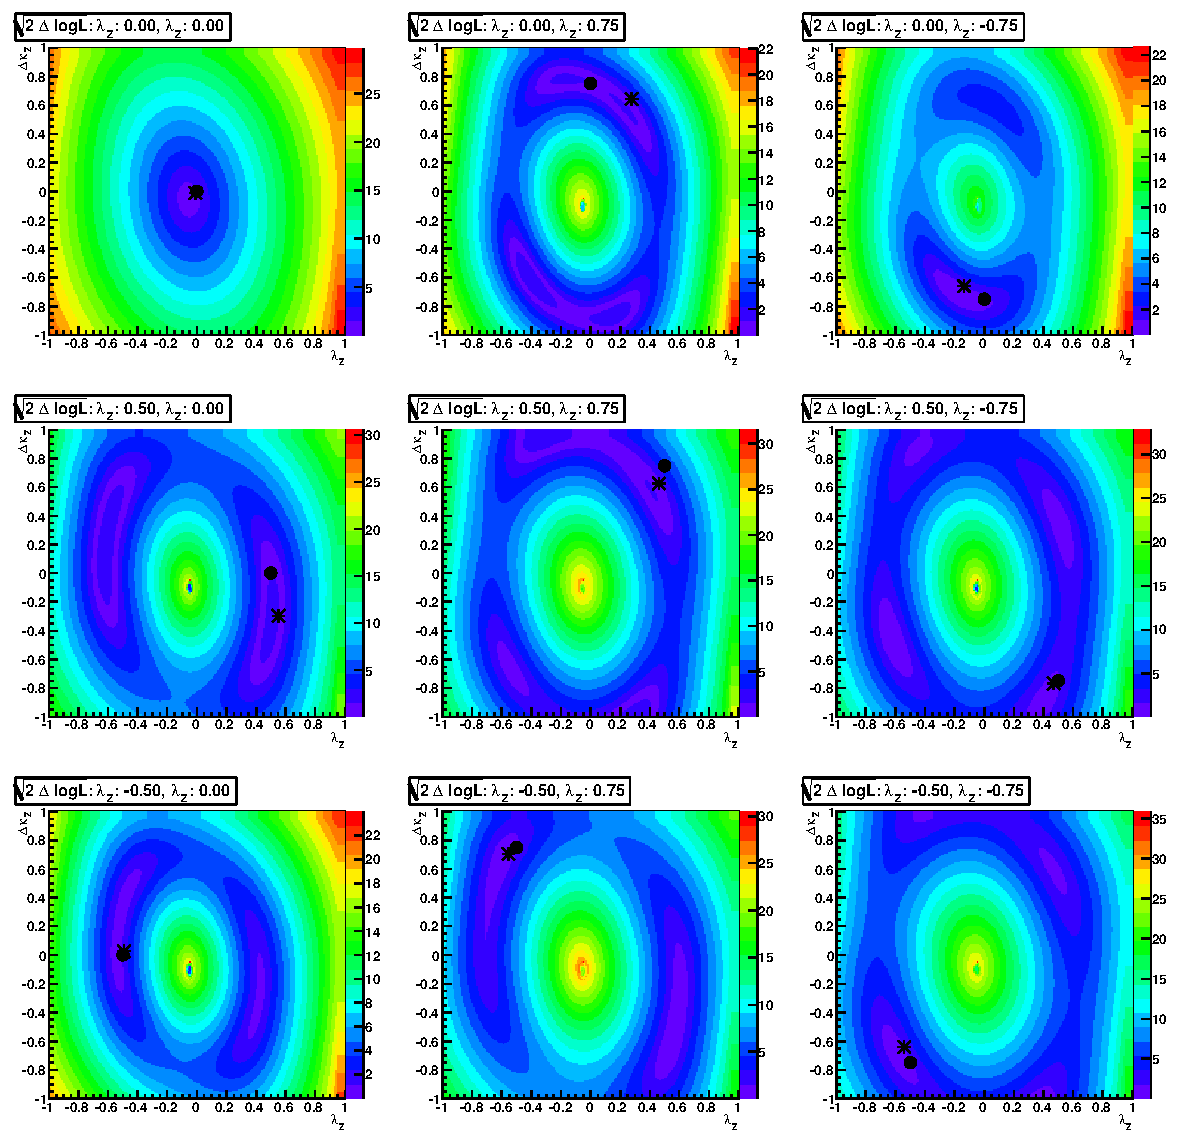
\includegraphics[width=1.0\textwidth]{figures/validation_likelihood_scans}
  }

  \caption[Likelihood scan for Signal Monte Carlo] {Likelihood scans
    for 350/pb of data excluding backgrounds. The curves
    represent the $\sqrt{2\Delta\log L}$ 1D significance of the difference between the
    likelihood with the sample's true anomalous couplings and the other
    values on the plain. The black star is the fit result when both couplings are
    allowed to float in the fit. The black point is the true value of the couplings.}
  \label{fig:val_scans}
\end{figure}

\begin{figure}[tp]
  \centerline{
    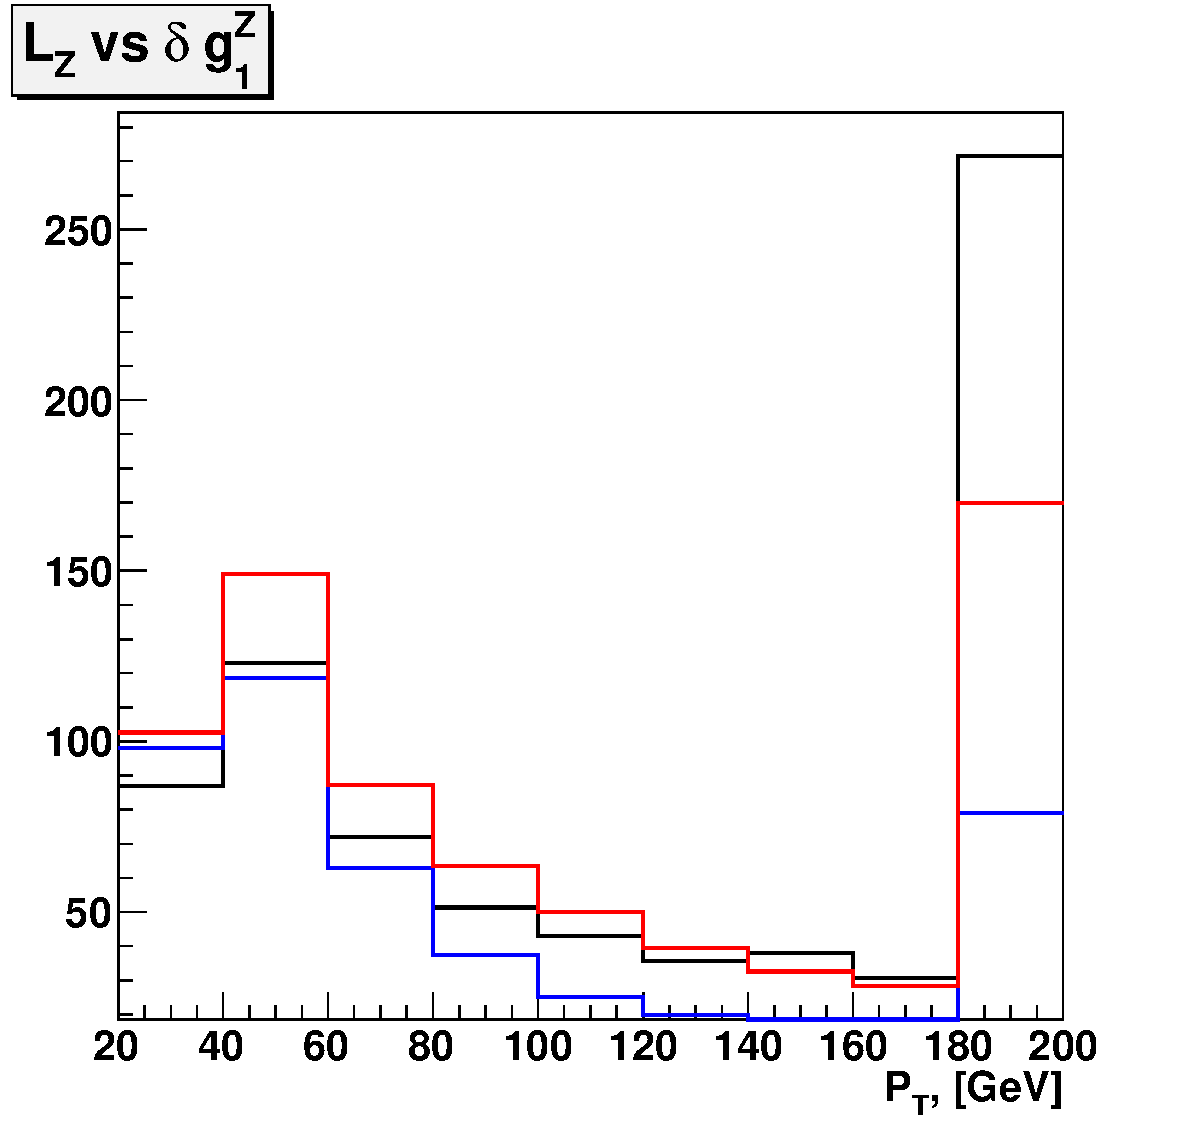
\includegraphics[width=0.6\textwidth]{figures/lz_vs_dkg}
  }

  \caption[Leading lepton pt shape for different couplings]{The
  leading lepton \pt\ distributions for events with $\lambda_{Z}=0.5$
  (black), $\Delta g^Z_1=0.5$ (blue) and $\Delta g^Z_1=0.75$
  (red). The distributions are generated by MCFM at NLO applying
  kinematical selection requirements used in the analysis.} \label{fig:lz_vs_dkg}
\end{figure}

\subsection{Toy Monte Carlo studies}
Figure~\ref{fig:toys} shows results of the fits
performed in toy Monte Carlo studies of the fit model. In each toy
experiment the PDF that is used to fit aTGC is used to generate the
leading lepton \pt\ distribution with the nominal number of \WW\
events expected. The normalization is treated as a nuisance parameter
and left free floating in the fit. The distributions of fitted
anomalous couplings are shown for 1000 toy experiments.

Figure~\ref{fig:fulltoys} shows the toy Monte Carlo studies using full
PDF setting all anomalous couplings to zero during generation and
letting them free in the fit. The results can be used to estimate the
expected uncertainties on the couplings: $\sigma(\lambda_{Z})=0.022$,
$\sigma(\Delta g^Z_1)=0.038$ and $\sigma(\Delta\kappa_\gamma)=0.088$.

From these studies we find no bias in the fitter. 

\begin{figure}[tp]
  \centering
    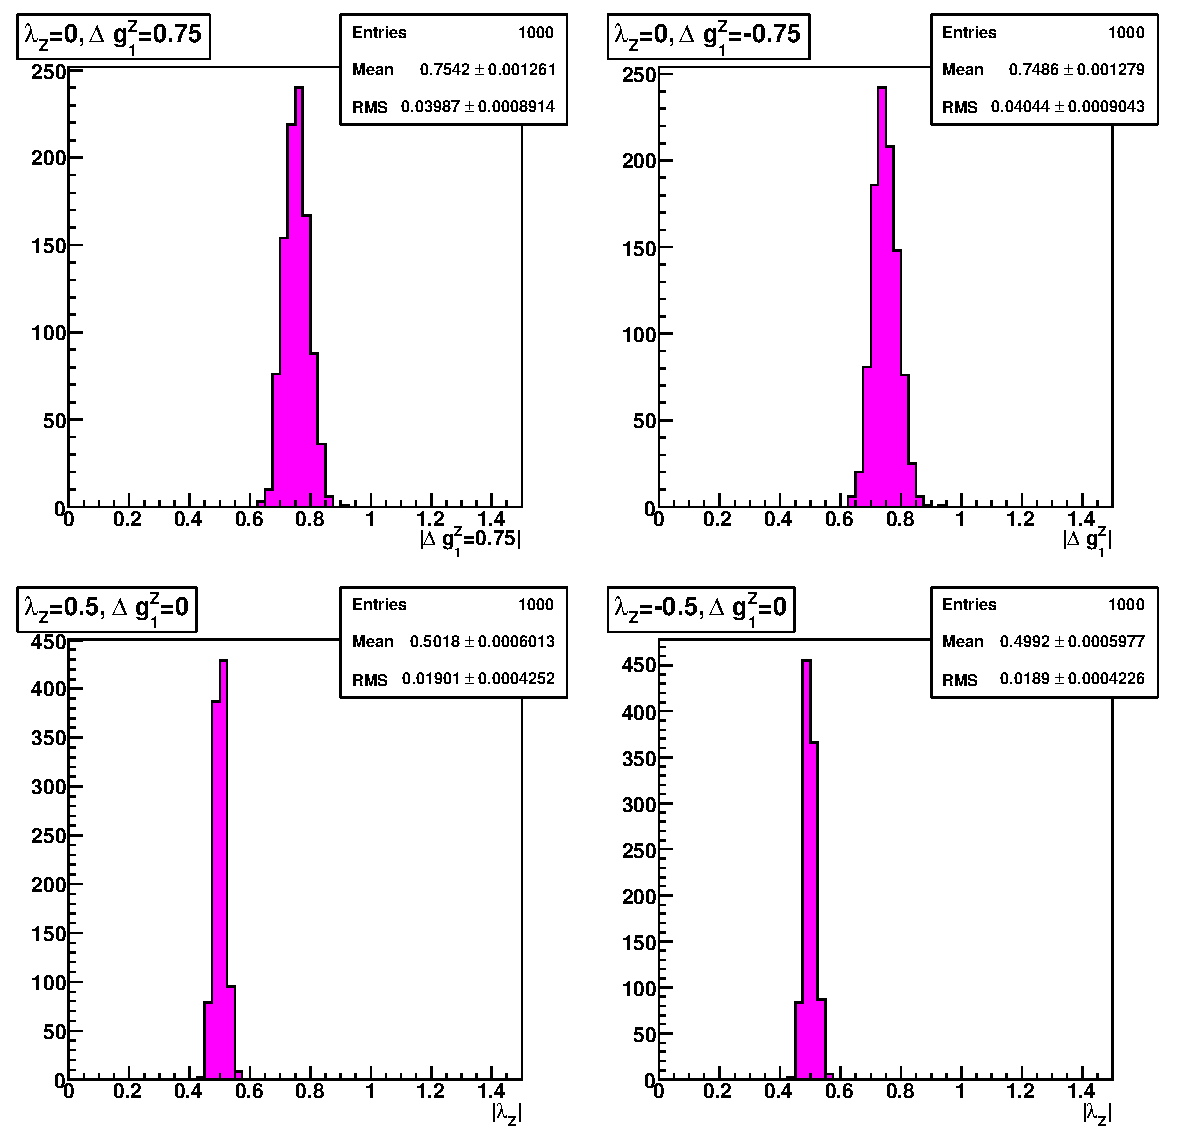
\includegraphics[width=0.8\textwidth]{figures/fit_wwATGC_toymc_1D_abs}
    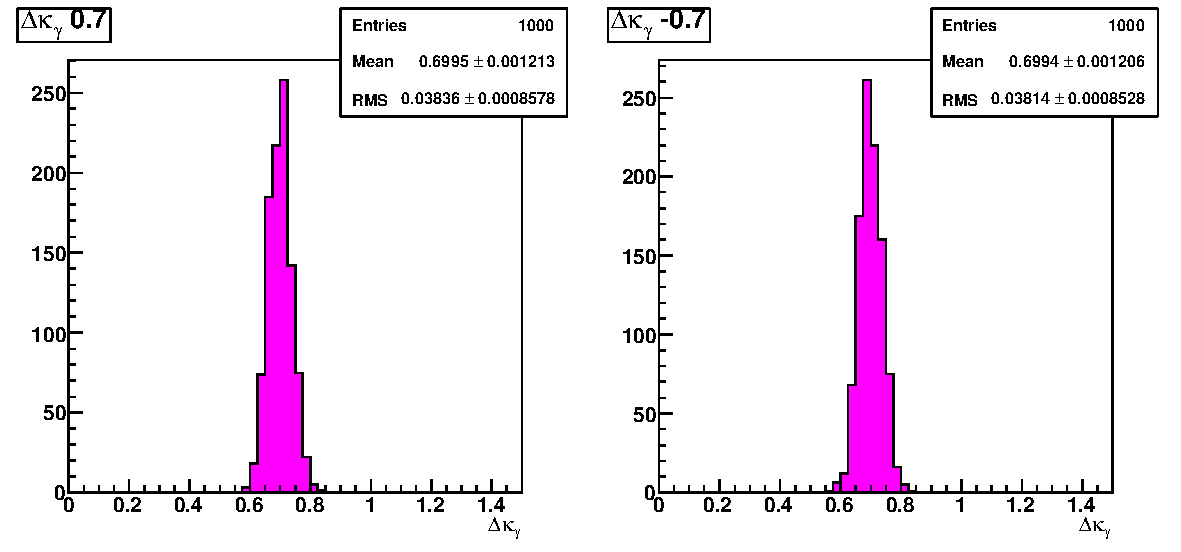
\includegraphics[width=0.8\textwidth]{figures/fit_wwATGC_toymc_1D_abs2}

  \caption[Toy Monte Carlo studies] {Fit results for 2-dimentional
  $\lambda_{Z}$-$\Delta g^Z_1$ (top) and
  $\lambda_{Z}$-$\Delta\kappa_\gamma$ (bottom) aTGC models using toy
  Monte Carlo experiments in which the leading lepton \pt\
  distribution is generated from the signal PDF with non-zero
  anomalous couplings. Backgrounds are excluded from the fits.}

\label{fig:toys}
\end{figure}

\begin{figure}[tp]
  \centering
    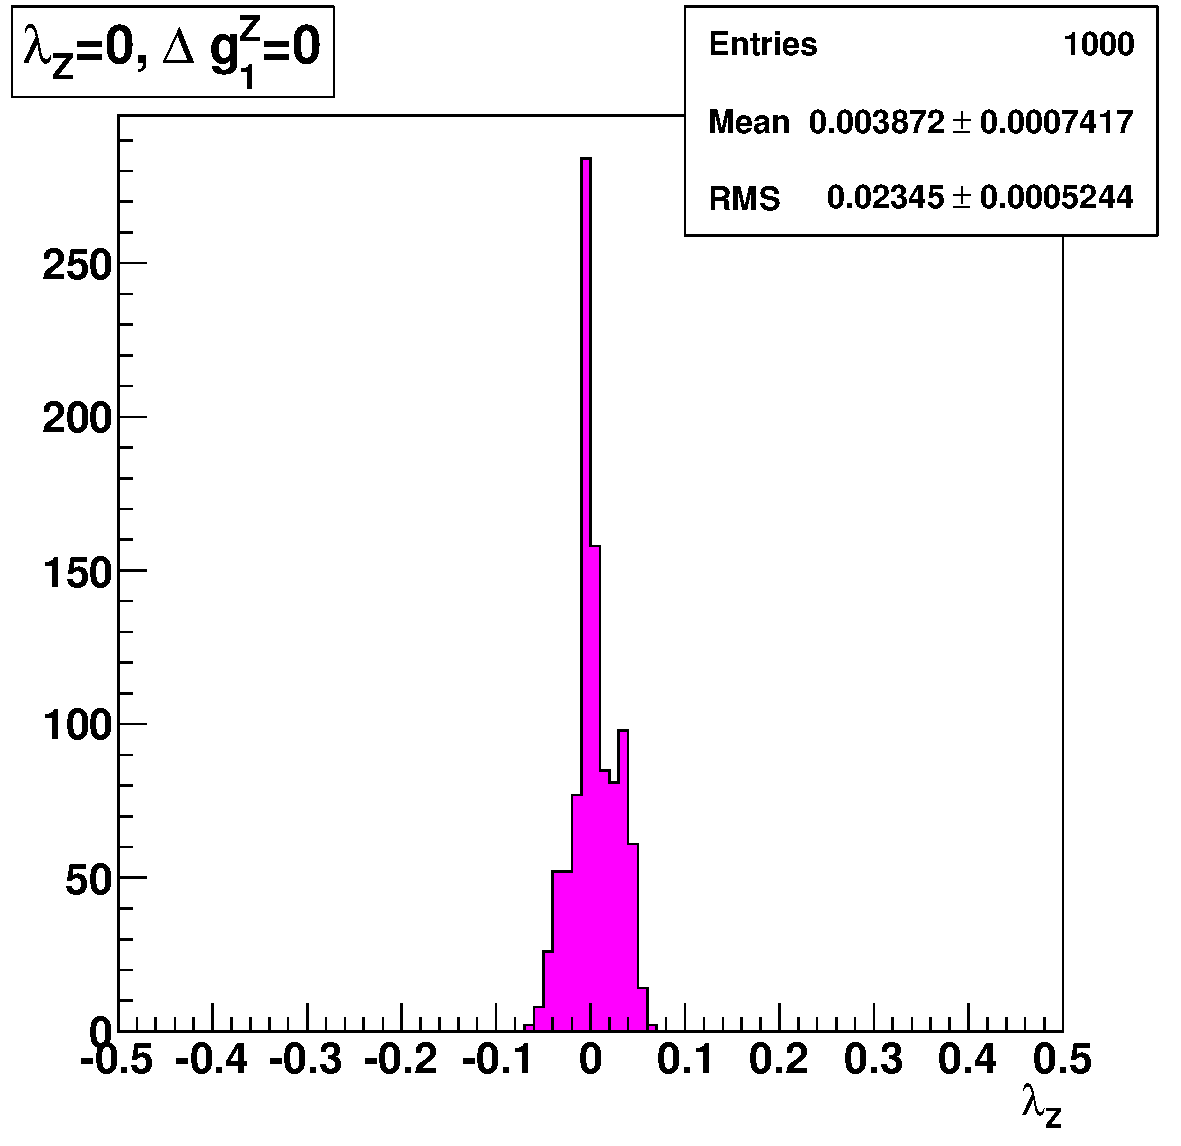
\includegraphics[width=0.3\textwidth]{figures/fulltoy_lz.pdf}
    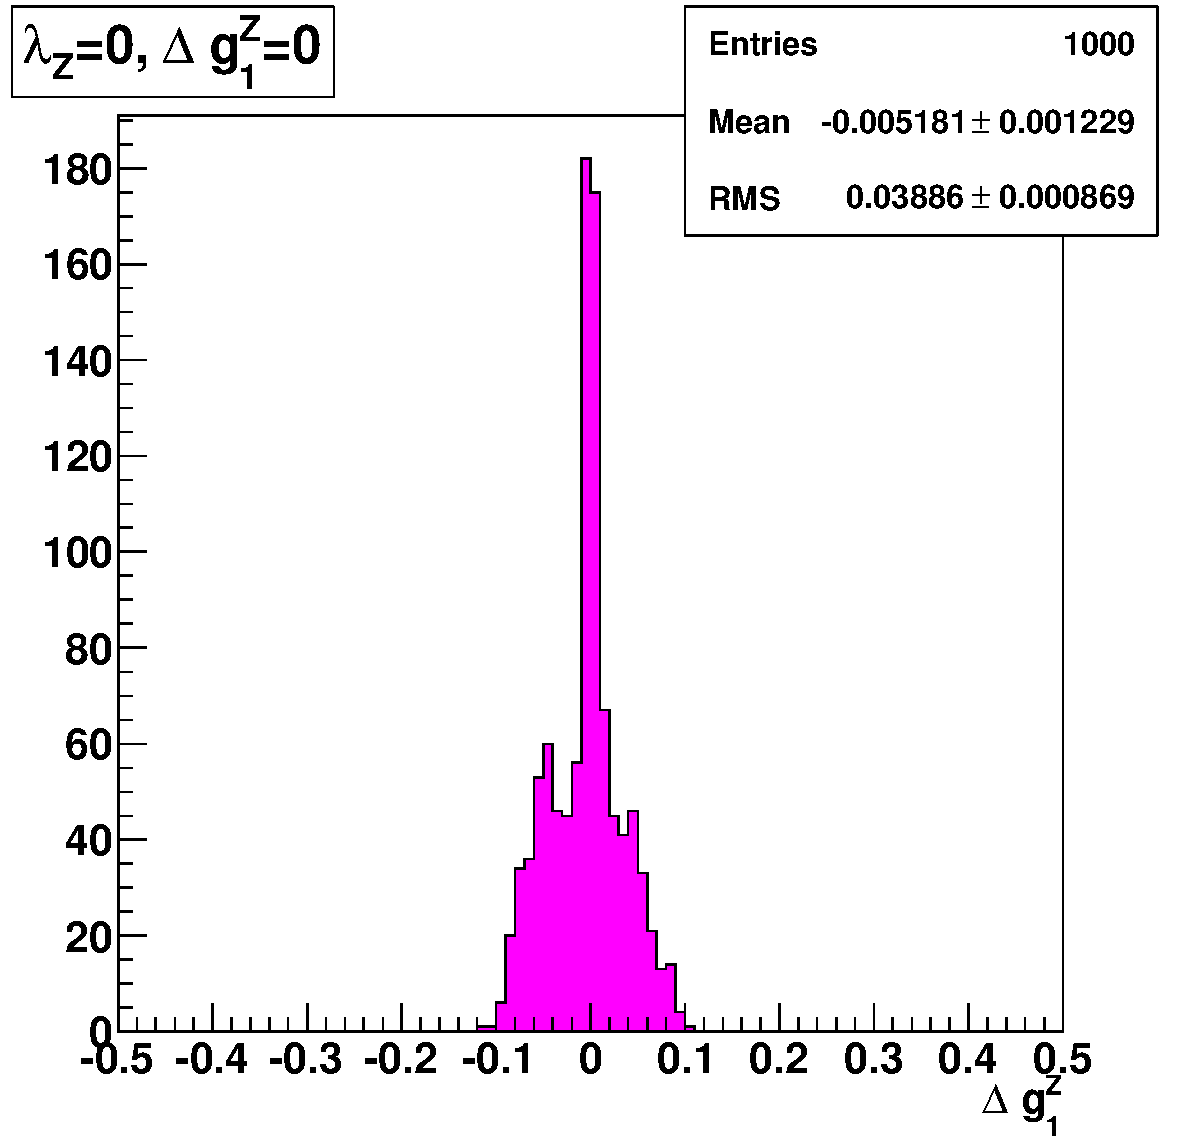
\includegraphics[width=0.3\textwidth]{figures/fulltoy_gz1.pdf}
    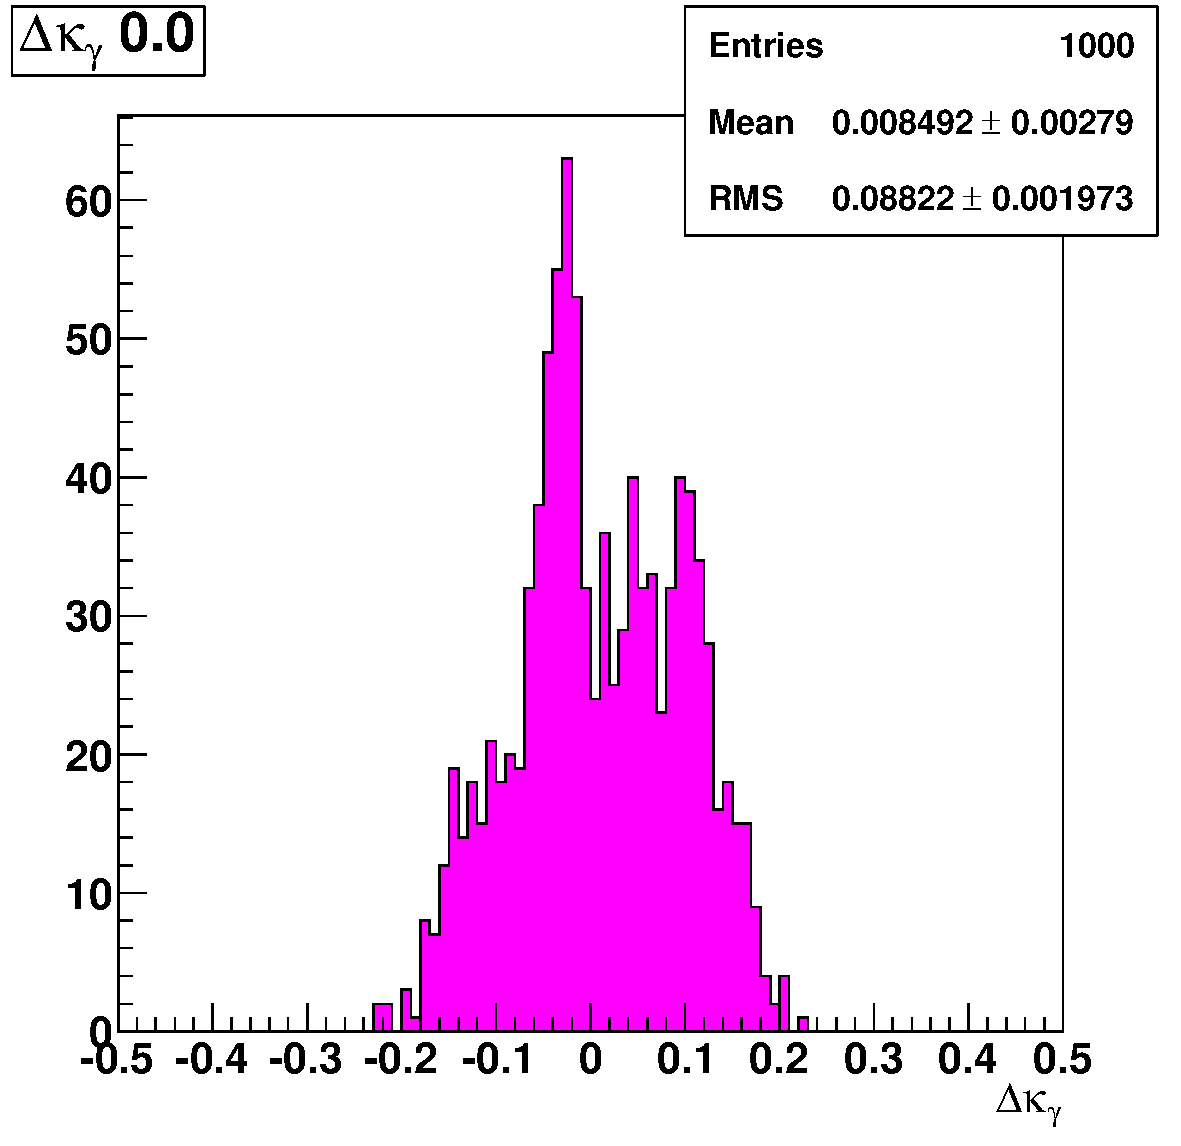
\includegraphics[width=0.3\textwidth]{figures/fulltoy_kg.pdf}

  \caption[Expected uncertainties]{Fits for anomalous couplings using
  the leading \pt\ distribution generated with zero anomalous
  couplings using toys Monte Carlo trials}

\label{fig:fulltoys}
\end{figure}


\subsection{Pseudo-experiments}
Figures~\ref{fig:fit_ww_mc_1D} and \ref{fig:fit_wwATGC_mc_1D_abs} show
results of the fits on \ww\ Monte Carlo samples with and without
anomalous couplings and excluding backgrounds. If only one coupling is
fitted it is not possible to get the sign right, so only absolute
values can be measured.

Pseudo-experiments with Standard Model \ww\ Monte Carlo are performed
to look for bias in the fit for the central value and to test the
uncertainty estimation. No significant deviation from zero is
found. Pseudo-experiments with non-zero anomalous couplings show
results consistent with anomalous couplings used to generate the
samples.

These tests conclude that the modeling of the leading lepton \pt\
distribution in terms of anomalous couplings does not lead to any
sizable deviation and the model can be used to measure anomalous
couplings in data.

\begin{figure}[tp]
  \centering
    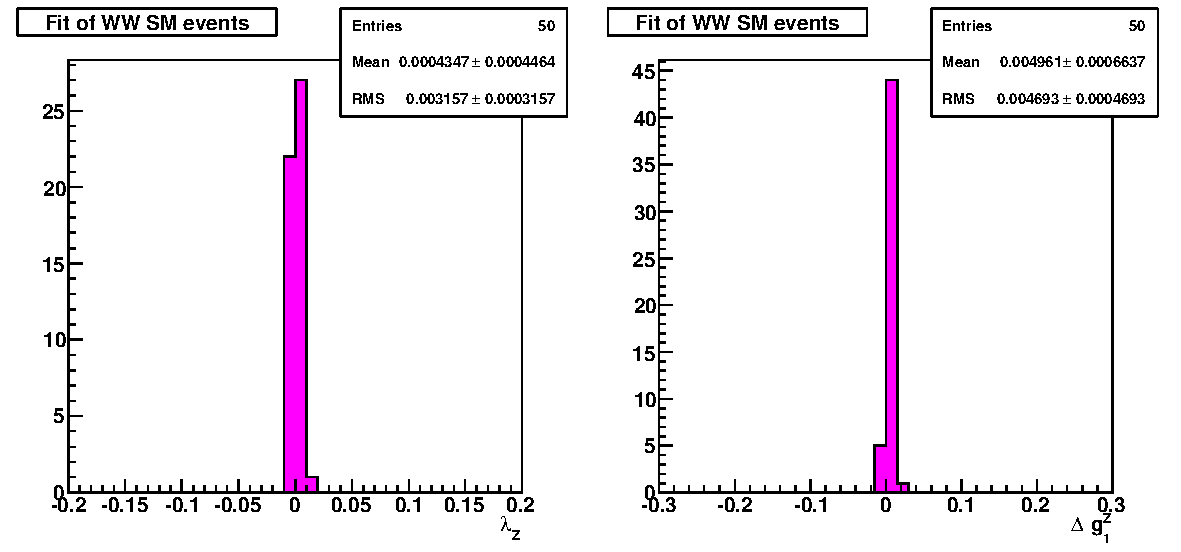
\includegraphics[width=1.0\textwidth]{figures/fit_ww_mc_1D}
    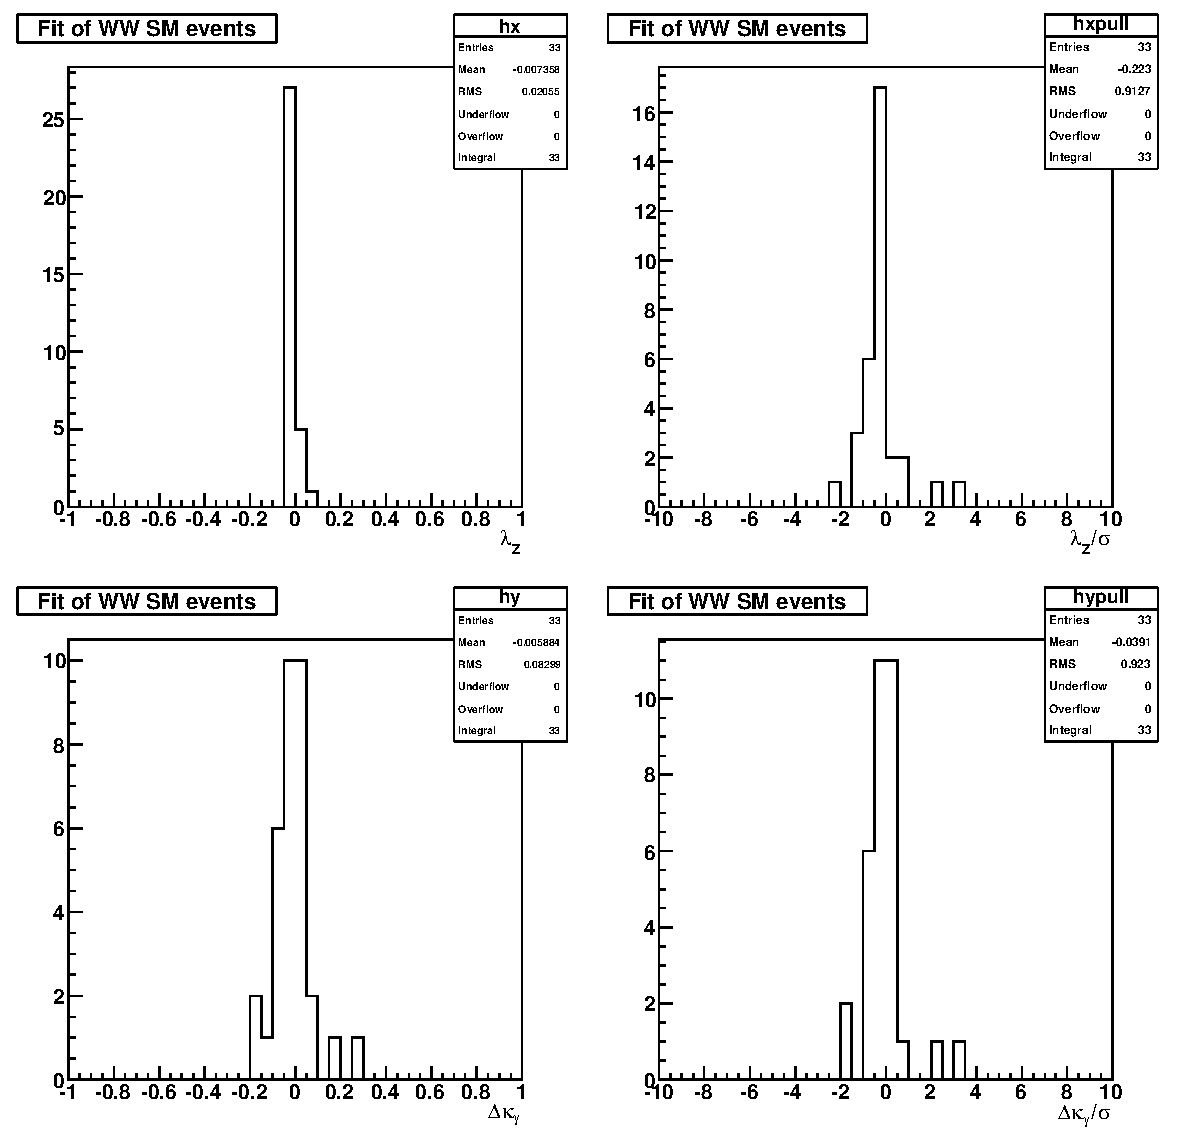
\includegraphics[width=1.0\textwidth]{figures/fit_ww_mc_1D_2}

  \caption[1D fits to WW SM Monte Carlo] {Fit results for
  2-dimentional $\lambda_{Z}$-$\Delta g^Z_1$ (top) and
  $\lambda_{Z}$-$\Delta\kappa_\gamma$ (bottom) aTGC models using 50
  independent pseudo-data experiments made of Madgraph Standard
  Model \ww\ simulated data. Only one coupling floating in the fit,
  while the other one is fixed to the Standard Model
  value. Backgrounds are excluded from the fits.}

\label{fig:fit_ww_mc_1D}
\end{figure}


%% \begin{figure}[tp]
%%   \centerline{
%%     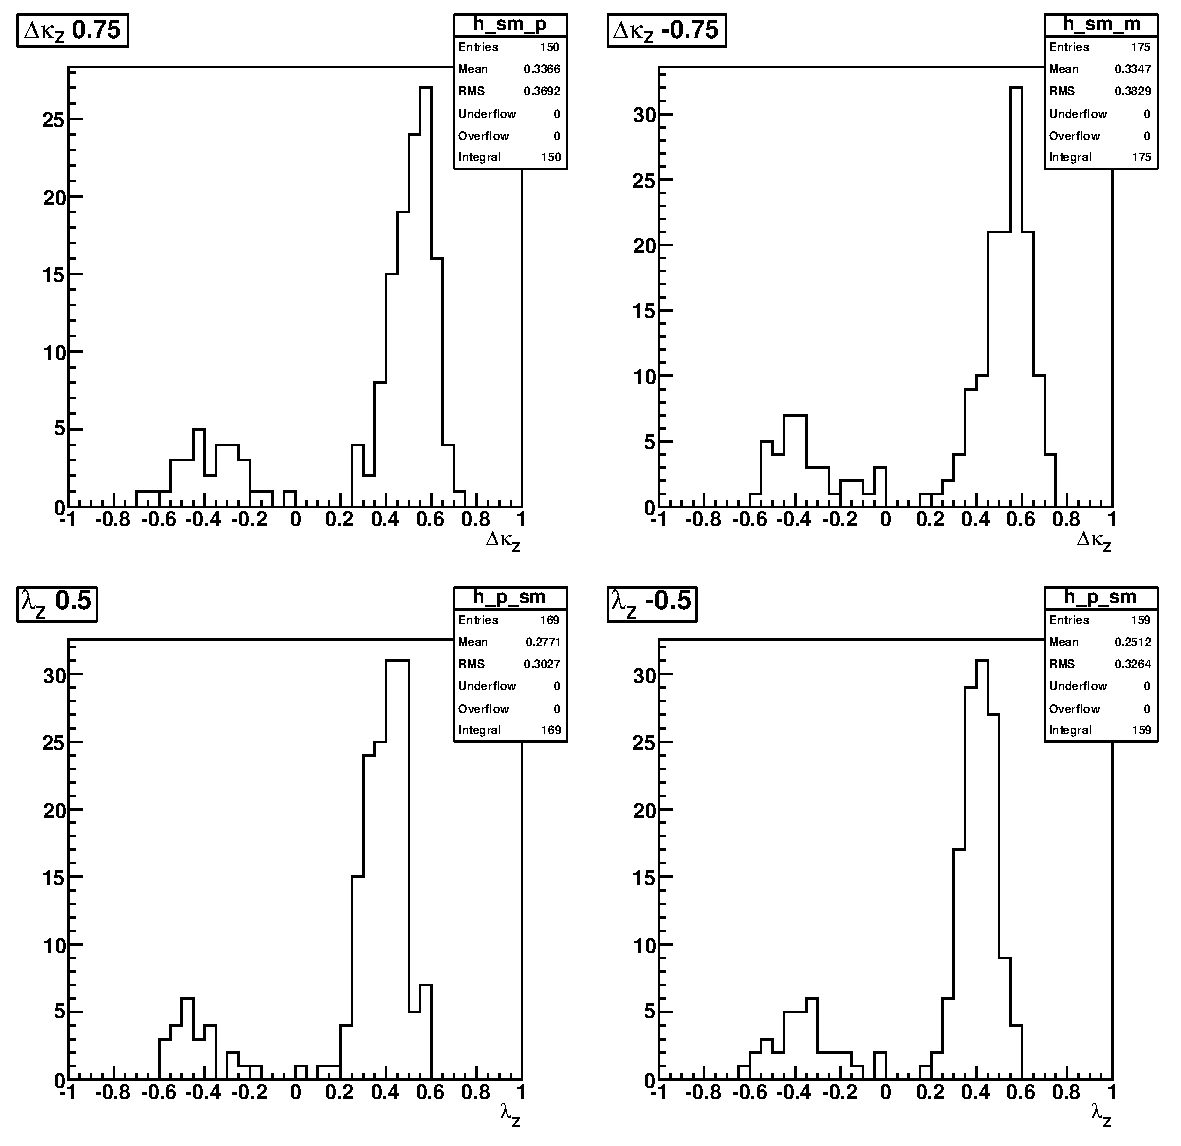
\includegraphics[width=1.0\textwidth]{figures/fit_wwATGC_mc_1D_pm}
%%   }

%%   \caption[1D fits to WW aTGC Monte Carlo] {Fits to WW Monte Carlo
%%     samples with anomalous couplings with 11 events in a sample. No
%%     background. Only one coupling is floated in the fit. Sign of the
%%     coupling cannot be determined in the fit.}
%%   \label{fig:fit_wwATGC_mc_1D_pm}
%% \end{figure}

\begin{figure}[tp]
  \centering
    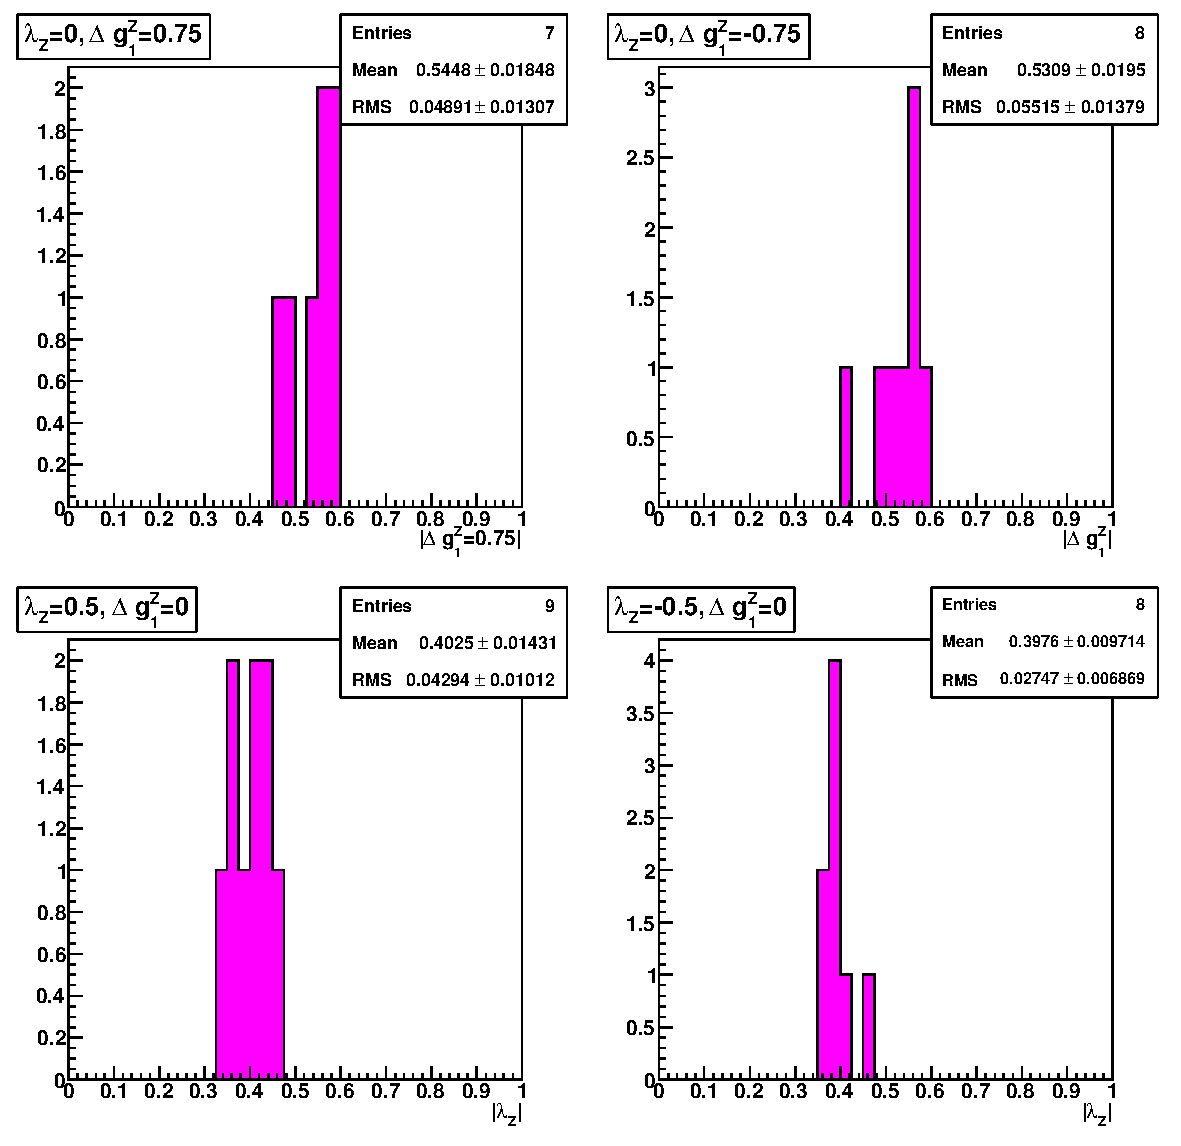
\includegraphics[width=0.8\textwidth]{figures/fit_wwATGC_mc_1D_abs}
    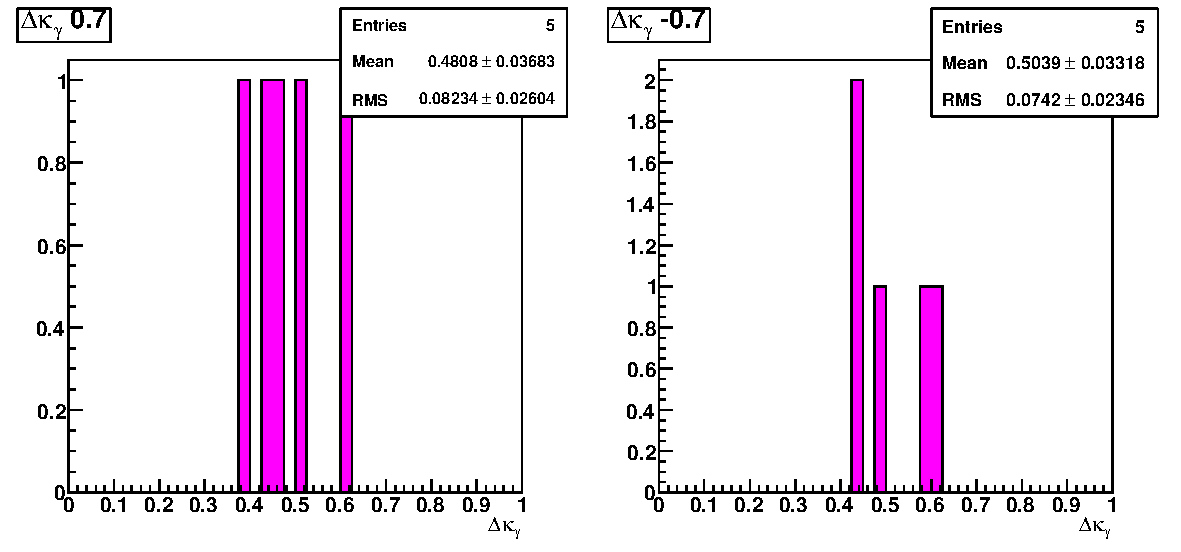
\includegraphics[width=0.8\textwidth]{figures/fit_wwATGC_mc_1D_abs2}

  \caption[1D fits to WW aTGC Monte Carlo] {Fits to $WW$ Monte Carlo
    samples with anomalous couplings. Pseudo-data experiments are made
    with 5-10 times lower number of events in each experiment due
    limited amount of simulated data. Backgrounds are excluded from
    the fits. Only one coupling is allowed to float in the
    fit. Absolute values of the couplings are  shown.}  
    \label{fig:fit_wwATGC_mc_1D_abs}
\end{figure}

\subsection{Fit on data}
We check how much the normalization of different components were
changed during the fit with respect to the inial values. For this test
we treat anomalous couplings as nuisance parameters and hide their
central values.

Table~\ref{tab:fit_yields} summarizes the fit results for event
yields. From it we conclude that the excess of the events that we
observed in the cross-section measurement is absorbed mostly in \ww\
event yield. Looking at the correlation matrix
Figure~\ref{fig:fit_correlations} one can see that there is
significant correlation between \ww{}, \wjets{} and \ttbar{} event
yields. Figure~\ref{fig:fit_data} shows a reasonable agreement of the
final fit pt distribution and the one observed in data. 

%% Minuit2Minimizer: Minimize with max iterations 4000 edmval 1 strategy 1
%% Minuit2Minimizer : Valid minimum - status = 0
%% FVAL  = -1578.2051799912831
%% Edm   = 2.84316661007704903e-06
%% Nfcn  = 177
%% n_dy	  = 14.2216	 +/-  6.60059	(limited)
%% n_top	  = 88.7706	 +/-  21.5922	(limited)
%% n_wjets	  = 86.5649	 +/-  19.9815	(limited)
%% n_ww	  = 915.148	 +/-  45.4547	(limited)
%% n_wz	  = 18.5309	 +/-  1.89849	(limited)
%% n_zz	  = 10.5487	 +/-  0.999248	(limited)
%% x_par	  = 0.00401641	 +/-  0.0229406	(limited)
%% y_par	  = 0.00828161	 +/-  0.0352541	(limited)
%% Minos: Lower error for parameter 0  :  -6.73027
%% Minos: Upper error for parameter 0  :  6.74416
%% Minos: Lower error for parameter 1  :  -21.6282
%% Minos: Upper error for parameter 1  :  21.6914
%% Minos: Lower error for parameter 2  :  -20.078
%% Minos: Upper error for parameter 2  :  20.0657
%% Minos: Lower error for parameter 3  :  -45.2995
%% Minos: Upper error for parameter 3  :  45.6166
%% Minos: Lower error for parameter 4  :  -1.9004
%% Minos: Upper error for parameter 4  :  1.89958
%% Minos: Lower error for parameter 5  :  -1.00008
%% Minos: Upper error for parameter 5  :  0.999759
%% Minos: Lower error for parameter 6  :  -0.0227218
%% Minos: Upper error for parameter 6  :  0.020276
%% Minos: Lower error for parameter 7  :  -0.0348234
%% Minos: Upper error for parameter 7  :  0.0323726


\begin{table}[!ht]
  \begin{center}
 {\small
  \begin{tabular} {|l|c|c|c|}
\hline
  Parameter       &   Initial value & Fit value & Global Correlation \\
\hline
  N$_{\ww}$       & $819.9\pm57.6$  & $915.1\pm45.5$ & 0.69 \\
  N$_{Top}$       & $121.6\pm23.4$  & $88.8\pm21.6$  & 0.52 \\
  N$_{\wjets}$    & $78.1\pm22.0$   & $86.6\pm20.0$ & 0.55 \\
  N$_{\wz}$       & $18.5\pm1.9$    & $18.5\pm1.9$   & 0.06 \\
  N$_{\dyll}$     & $11.7\pm6.8$    & $14.2\pm6.6$   & 0.22 \\
  N$_{\zz}$       & $10.6\pm1.0$    & $10.5\pm1.0$   & 0.03 \\
\hline
  \end{tabular}
  }
  \caption{Nominal fit parameter values.}
   \label{tab:fit_yields}
  \end{center}
\end{table}

\begin{figure}[tp]
  \centering
    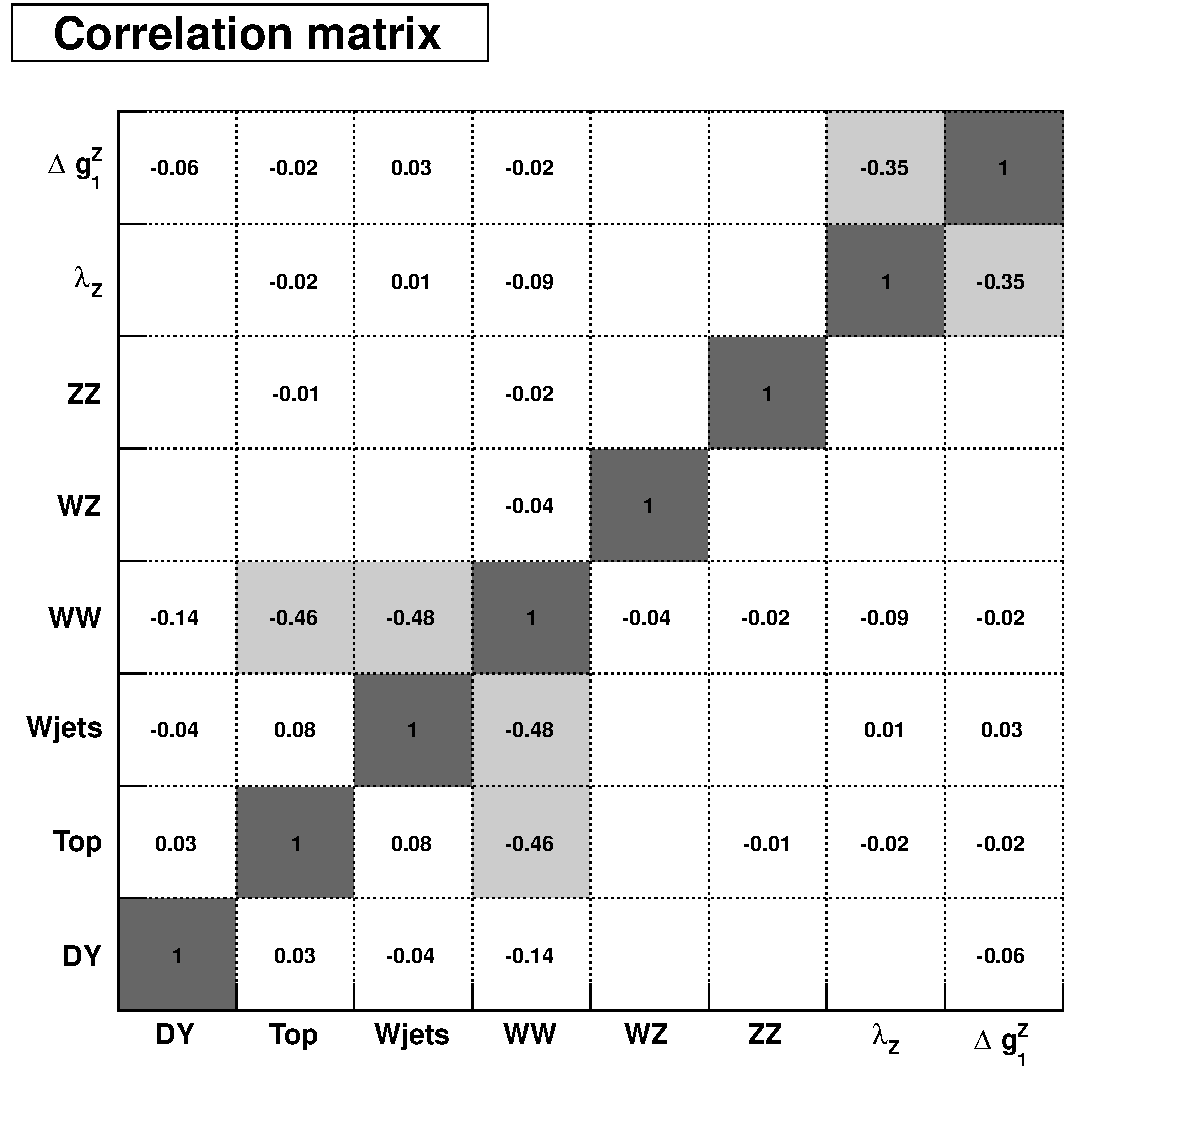
\includegraphics[width=.60\textwidth]{figures/correlations}

  \caption[Fit parameter correlations] {Correlation matrix for the nominal fit parameters.}
  \label{fig:fit_correlations}
\end{figure}

\begin{figure}[tp]
  \centering
    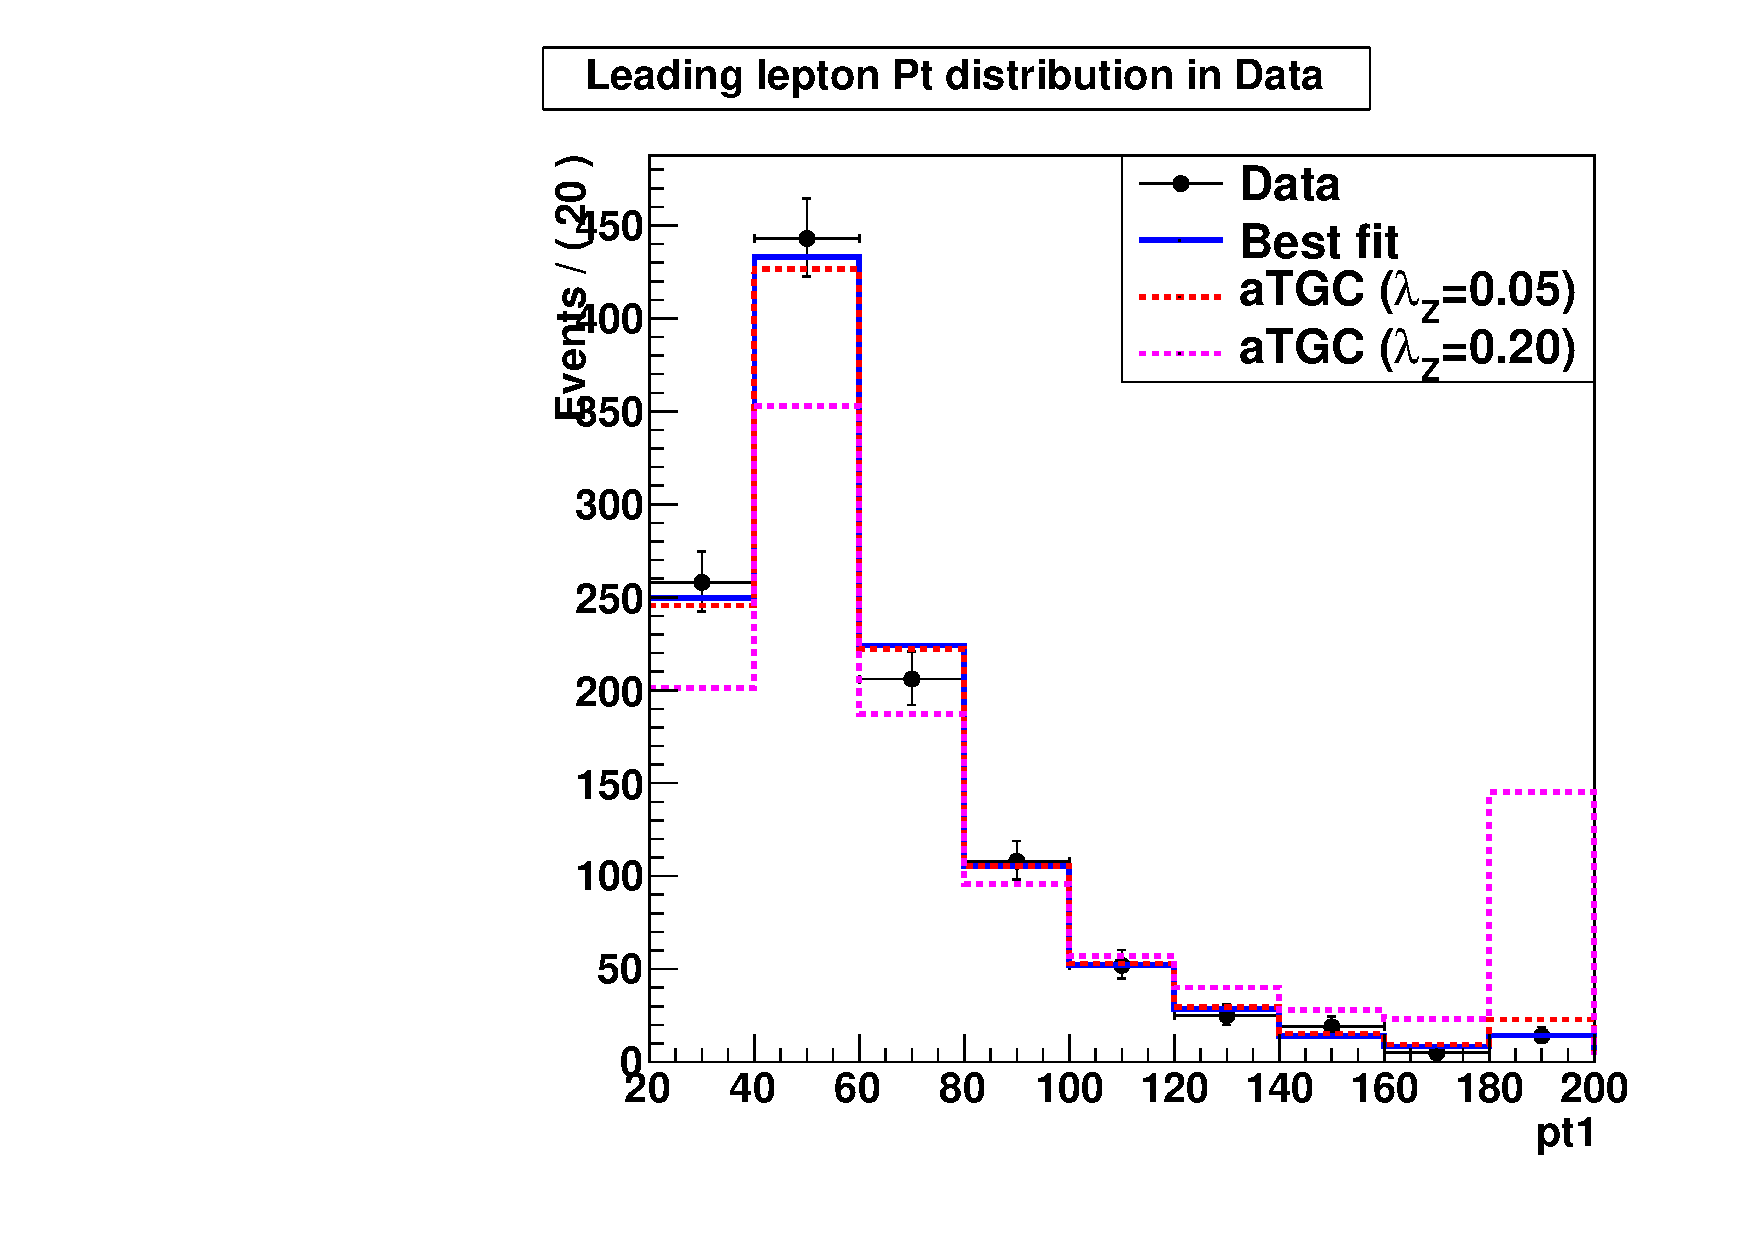
\includegraphics[width=.45\textwidth]{figures/lz_dgz_pdf_data}
    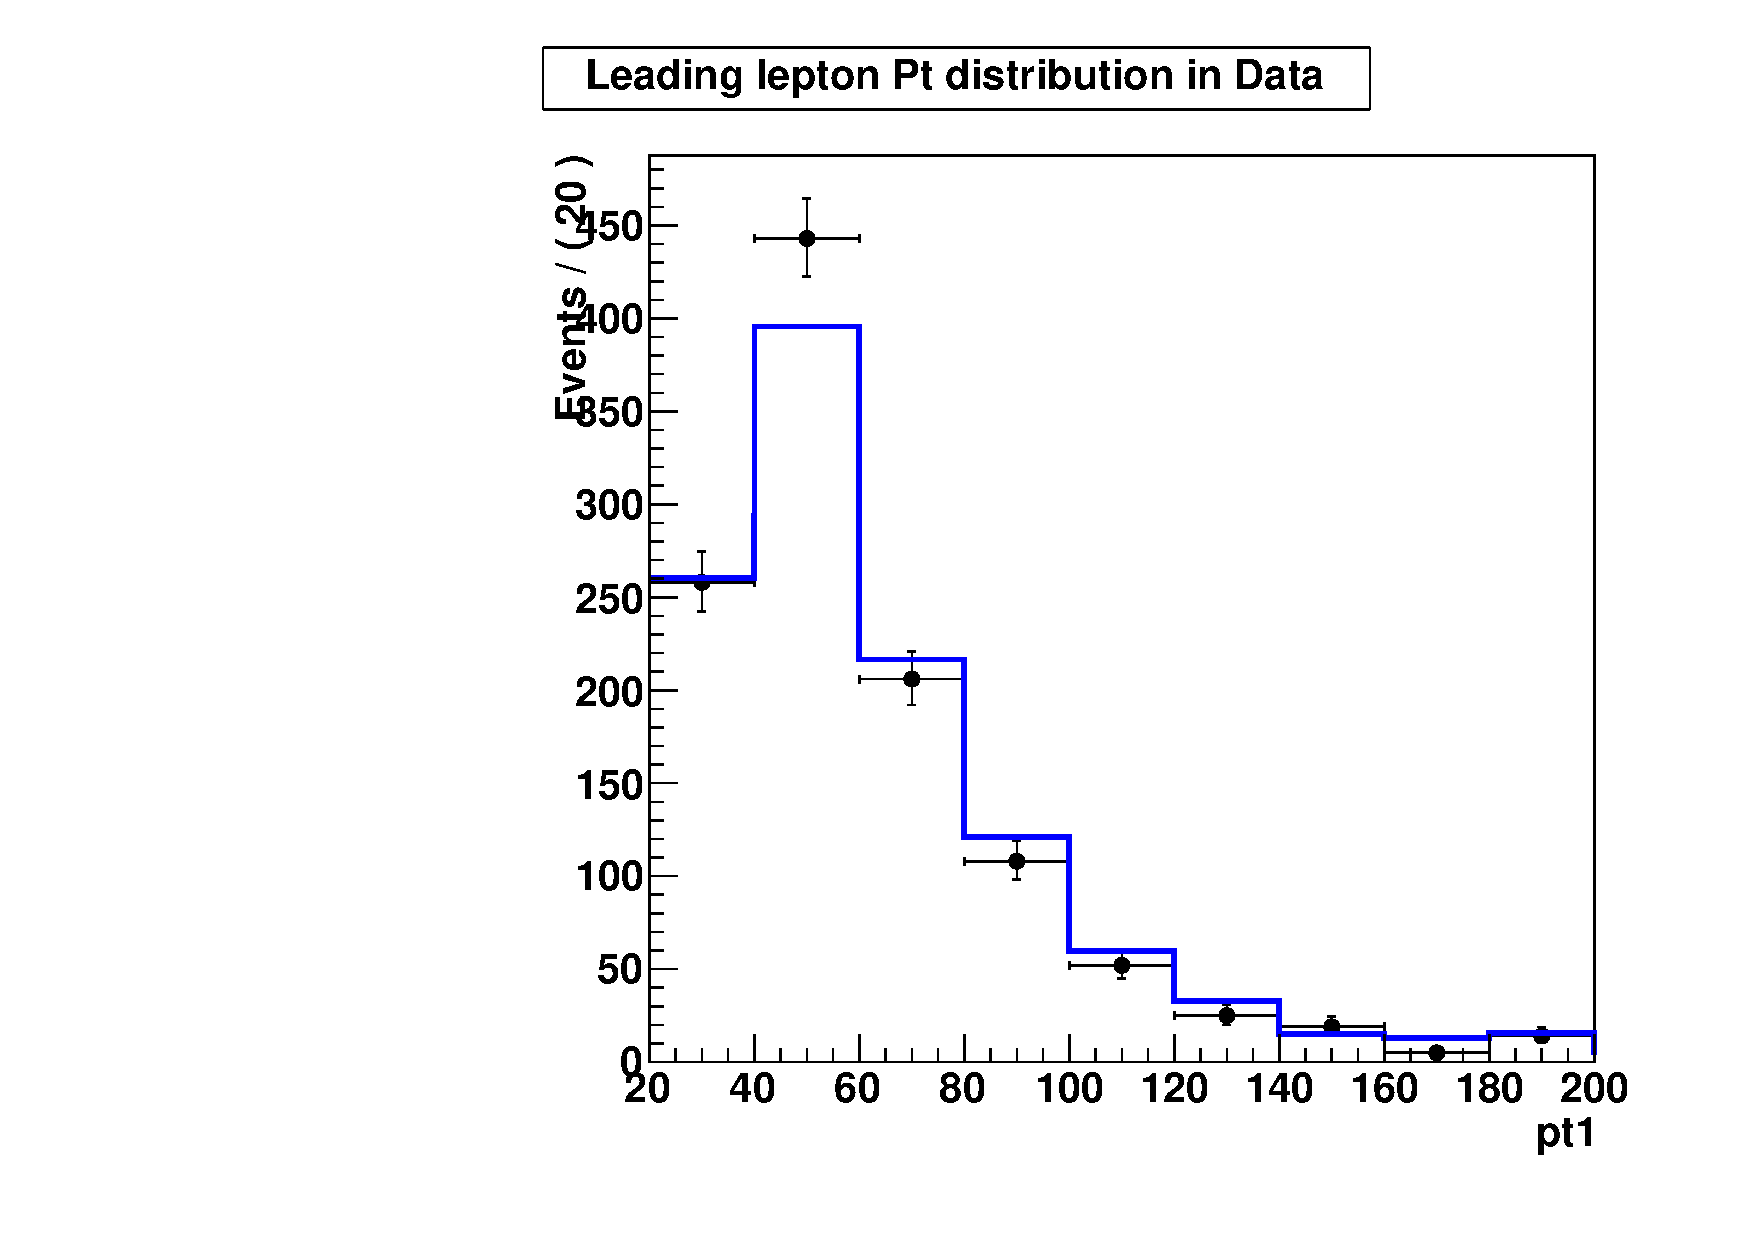
\includegraphics[width=.45\textwidth]{figures/lz_dkg_pdf_data}

  \caption[Fit on data] {Final combined pdf distribution (blue
  histogram) on top of observed data yield. Left plot shows results
  for a fit using $\lambda_Z$-$\Delta g^Z_1$ model and the right one
  shows that of $\lambda_Z$-$\Delta\kappa_{\gamma}$ model.} \label{fig:fit_data}
\end{figure}

\subsection{QCD and PDF uncertainties}
Figure~\ref{fig:qcd_pdf} shows the effect of QCD and PDF uncertainties on
the leading lepton \pt\ distribution. The effect on the anomalous
couplings is found to be negligible: $10^{-4}-10^{-5}$.

\begin{figure}[tp]
  \centering
    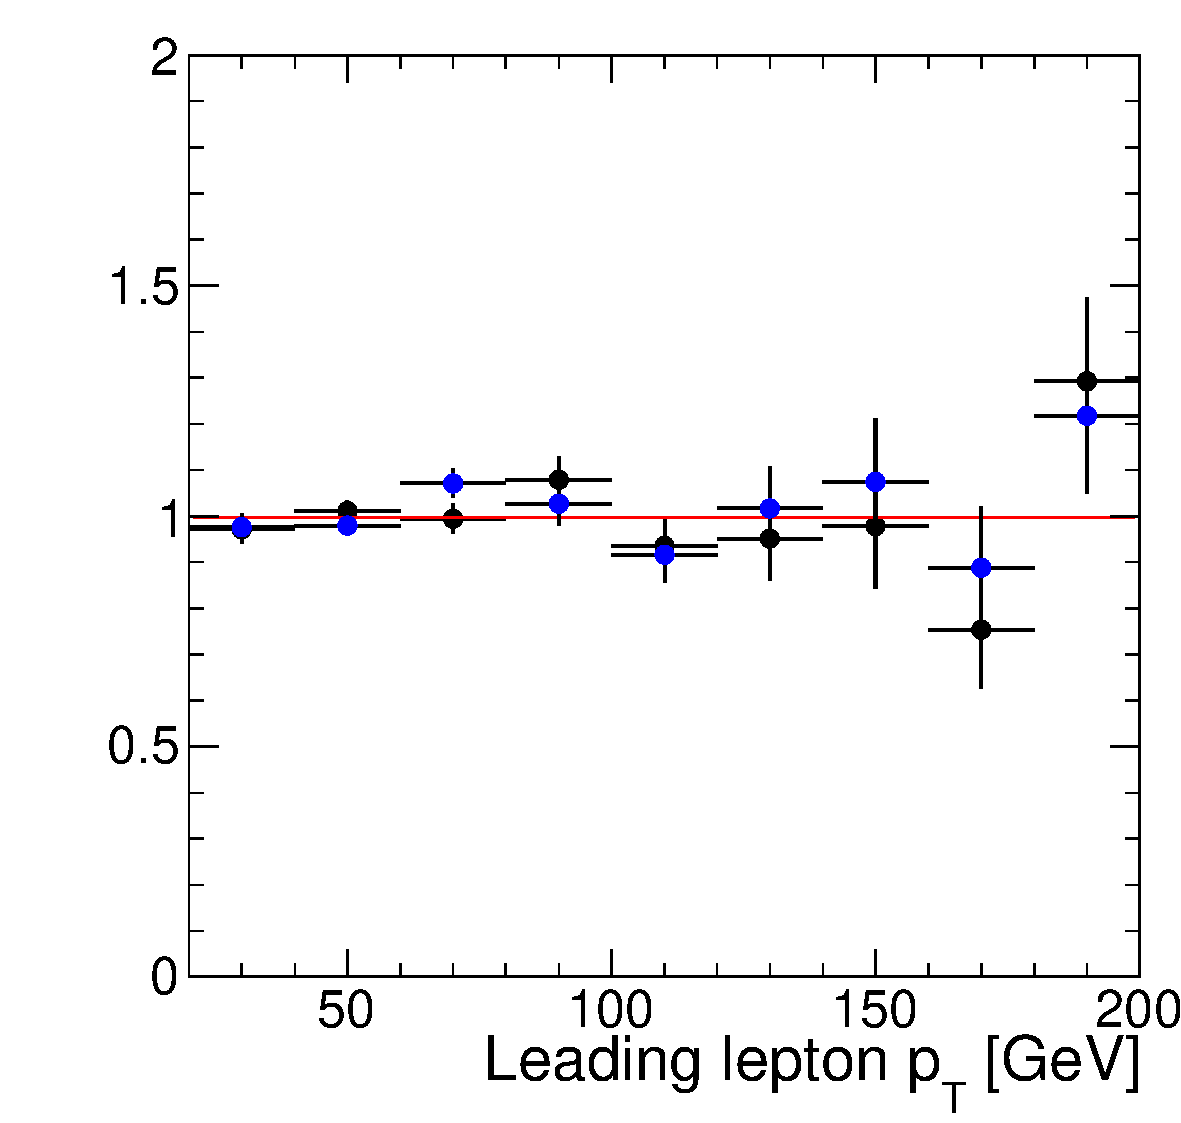
\includegraphics[width=.45\textwidth]{figures/qqww_qcd_uncertainties.pdf}
    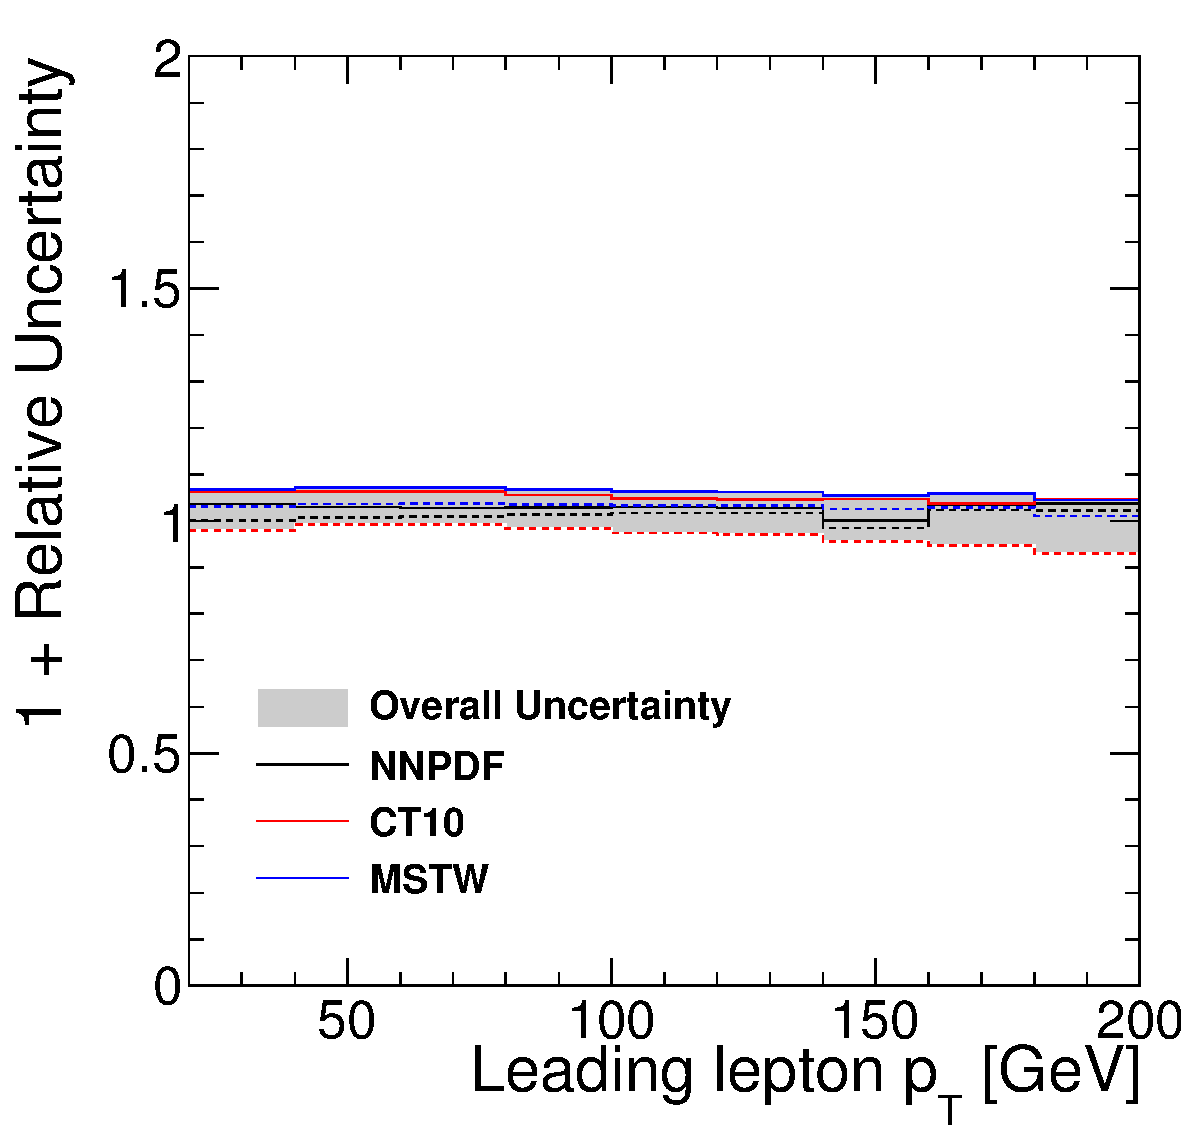
\includegraphics[width=.45\textwidth]{figures/qqww_pdf_uncertainties.pdf}

  \caption[QCD and PDF uncertianties]{QCD (left) and PDF (right)
  uncertainties on the leading lepton \pt\ distribution. The QCD plot
  shows a ratio of the distributions produced with MC@NLO
  generator at the nominal and up(black)/down(blue) QCD scales.} \label{fig:qcd_pdf}
\end{figure}
